\documentclass{standalone}
\usepackage{tikz}
\begin{document}
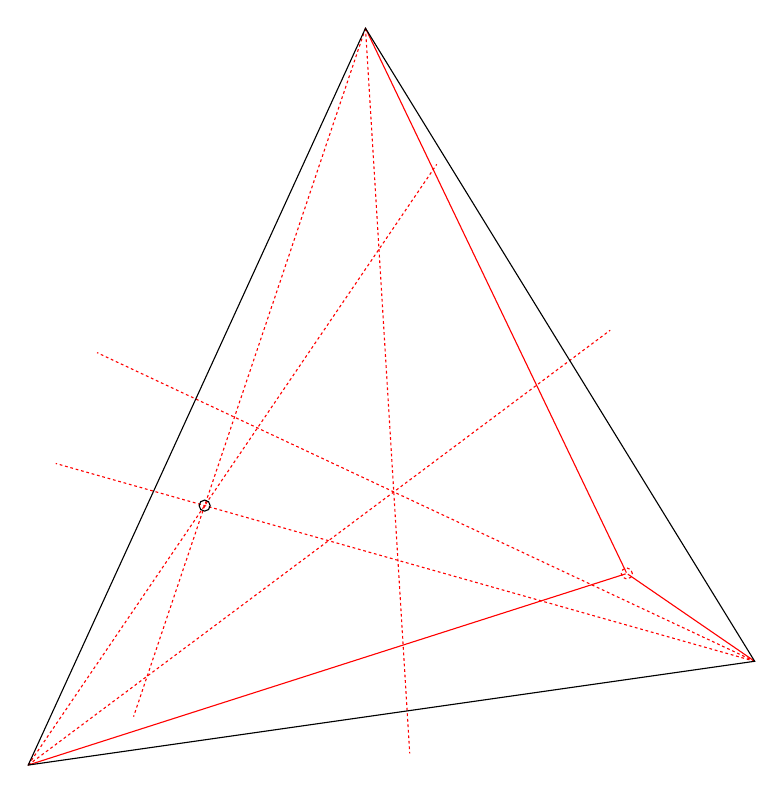
\begin{tikzpicture}[x=1pt,y=1pt]
\draw[red, dash pattern=on 1pt] (140.62,-15.00) -- (56.81,-263.77);
\draw[red, dash pattern=on 1pt] (281.25,-243.75) -- (28.69,-172.27);
\draw[red, dash pattern=on 1pt] (18.75,-281.25) -- (166.35,-64.20);
\draw[red, dash pattern=on 1pt] (140.62,-15.00) -- (156.60,-277.01);
\draw[red, dash pattern=on 1pt] (281.25,-243.75) -- (43.61,-132.23);
\draw[red, dash pattern=on 1pt] (18.75,-281.25) -- (229.05,-124.12);
\draw[red] (140.62,-15.00) -- (234.90,-211.72);
\draw[red] (281.25,-243.75) -- (235.42,-212.27);
\draw[red] (18.75,-281.25) -- (234.64,-212.15);
\draw (140.62,-15.00) -- (281.25,-243.75) -- (18.75,-281.25) -- cycle;
\draw[red, dash pattern=on 1pt] (235.05,-212.02) circle (2.00);
\draw (82.50,-187.50) circle (2.00);
\end{tikzpicture}
\end{document}
